% Intro to Intro - What is this about? {{{ 

The Smoluchowski coagulation equation provides a framework for modeling the temporal evolution of 
a particle group's distribution of masses under the influence of particle collisions and 
possible merge or fragmentation events. 
As such, it can be used to study the coagulation of particles in young circumstellar disks,
and the role dust plays in the early phases of planetary formation. \\

Previous studies of dust particle coagulation built using the Smoluchowski equation have made the 
simplifying assumption that the individual dust particles can be characterized entirely by the 
value of their mass (see e.g. 
    \cite{birnstiel_dullemond_brauer_2010}, 
    \cite{dullemond_dominik_2004}). 
This is due to the fact that the numerical integration of the Smoluchowski equation from one 
time step to the next involves the evaluation of a summation over the coagulation kernel. 
The inclusion of a second attribute like, for instance \textit{particle porosity}, greatly 
increases the dimensionality of the kernel, which leads to a significant increase in the 
computational cost required for the integration. \\

In this thesis we explore the possibility of lowering this computational cost via a stochastic 
Monte Carlo sampling of the kernel matrix. The central idea is to include only the most 
relevant sum terms, where relevance is determined by both the rate of a given collision,  
as well as by the effect it will have on the particle mass distribution function. \\

As of this writing, the question of how planets come into being is still far from solved. \\

... \\

It is widely accepted that dust plays an important role in early phases of planet formation. \\

This is not the same kind of dust one would find under a couch.
The dust that can be observed in the expanse between the stars 
and in proto-planetary disks ... [what kind of dust?] \\

When studying planet formation, it is desired to have 
a decent model for how the distribution of differently 
sized dust particles evolves with time. \\

One such model is given by the Smoluchowski coagulation equation, which a large part of this 
thesis will be built upon. 

% }}}
% Thesis Structure {{{ 
\section{Structure of this Thesis}

The thesis is structured as follows: \\

We will start by giving a short overview of a number of widely accepted ideas
related to the origin and formation of planets in \cref{sec:prerequisites}. \\

After that, we will continue with the definition of a simplified model for a proto-planetary
disk in \cref{ch:disk}. The model should include the most relevant properties of both the disk and 
its gas and dust contents. It will be used to model the dust particle kinematics and define the dust 
particle collision rates. \\

In \cref{ch:smoluchoswki} we will then utilize the Smoluchowski coagulation equation to build a 
simplified model of the dust particle mass distribution, as well as its temporal evolution under 
the influence of particle collisions and the following associative/disassociative events. 
The definition of a dust coagulation model will involve the discretization of the mass axis, 
the definition of a kernel matrix for both coagulation and fragmentation processes,
as well as the integration of the Smoluchowski equation. \\

Having constructed the complete kernel matrix, in \cref{ch:sampling} we will focus on the 
implementation of stochastic Monte Carlo sampling of the kernel. 
Here the task is to identify the most relevant collisions at a certain point in time,
define a sensible probability density from that, 
and conduct a random sampling of all possible collision.

% }}}
% AAAAAAA {{{ 
\section{Short Introduction to Planet Formation}
\label{sec:prerequisites}

    % The following attempts to provide a brief overview of a number of widely accepted ideas 
    % that are central to mankind's understanding of the origin and formation of the universe 
    % and planets within it:

    Directly after the Big Bang, the conditions in the young universe were not favorable for the
    formation of large-scale structures. Extremely high temperatures prevented the agglomeration 
    of smaller constituents into more complex particles. \\

    Current consensus has it that it took approximately 380.000 years for
    the initial hot quark-gluon plasma to be cooled down sufficiently by 
    the expansion of the universe to enable 
    the creation of the first hadronic matter via 
    a combination of multiple quarks into one particle. 
    For us, the most relevant of these quark combinations were of course the proton and the neutron,
    as they provided the building blocks for the nuclei of the first atoms. \\

    The capture of electrons by these atomic cores lead to the creation of neutral atoms. 
    The elemental composition of the early universe was dominated by the contribution 
    of hydrogen present in the form of molecular gas and, to a lesser extent, 
    helium and trace amounts of metals. 

    % The birthplace of both stars and planets is widely accepted to found in giant 
    % interstellar clouds made up of large amounts of this gas.

    % find its origin in the 
    % collapse 
    % Large clouds consisting almost entirely ($>99\%$ by mass)

    % The results 
    

    % The products of the above-mentioned process can be seen in the large-scale spatial 
    % structure and chemical composition 

    % large clouds of gas

    % nebular hypothesis
    % collapse of gas cloud into disk

    % formation of star at center of disk

    % disk around star


              % the elemental composition of which
              % the distribution of which would be 
              % dominated by hydrogen and, to lesser extent, helium.
    
    % \begin{itemize}
    %     % \item 

    %           % "Modern NASA telescopes/observations "

    %           % via $\text H^+ + e^- \to \text H$,
    %           % and 
    %           % $\text H + \text H \to \text H_2$

    %           % as the cores in the subsequent formation of atomic formation.
    %           % into mostly hydrogen and, to a lesser 
    %           % extent, helium lead to the formation of the large scale chemical make-up of the 
    %           % universe that is still observed today.

    %     % \item formation of molecules ($\text{H}_2$ hydrogen gas)

    %     \item formation of stars (then fusion, $pp$-chain)
    %     \item in star: formation of heavier elements (up to iron)
    %     \item ejection of heavy elements out of star (supernova, other "flux?/transport?")

    %     \item int cooler regions: formation of small dust particles 
    %           Not the same kind of dust that accumulates under your bed. \\
    %           \todo{What kind of dust? [cite]} \\
    %           Small dust particles are held together by van-der-Waals or Coulomb forces.
    %     \item dust coagulation into larger structures
    %     \item fragmentation barrier
    %           Dust kinematics is influenced by both systematic and stochastic processes. \\
    %           (Keplerian motion, radial/azimuthal drift)
    %           (Brownian motion, turbulence)

    %     \item gas accretion
    %     \item mass accretion
    %     \item formation of planetary core
    %     \item in high-gas regions: formation of gas planets (like Jupiter, Saturn, Uranus, Neptune)
    %     \item in low-gas regions: formation of rocky planets (like Mercury, Venus, Earth, Mars)
    % \end{itemize}

% }}}
%     % The Interstellar Medium {{{
\clearpage\subsection{The Interstellar Medium}

    % What is the interstellar medium?
    The term \textit{interstellar medium} (ISM) is used to denote the matter and radiation that 
    can be found in the expanse of space between the stellar systems inside a galaxy. 
    As we will discuss further in the following sections, the ISM is widely considered to serve 
    as the birthplace of proto-planetary disks (PPDs), and subsequently, stars and planets. \\

    At first glance, it might not be easy to imagine how such giant objects like planets and 
    even stars can form in the ISM. After all, one might naively say that it consists of mostly
    nothing. From the point of view of a human living on Earth, the interstellar regions of
    outer space appear to be a near-perfect vacuum. \\

    Measurements of the the molcular particle number density in the ISM have been made in 
    previous studies by e.g. \cite{burton_2013}. Here, they showed that the number of particles 
    per unit volume can range from $\SI{1e16}{\meter^{-3}}$ all the way down to 
    $\SI{1e3}{\meter^{-3}}$. \\

    The exact value of the particle number density depends of course heavily on the precise 
    position in the ISM. Nonetheless, a comparison of the mere orders of magnitude involved 
    here demonstrates the huge difference in particle abundances in the ISM when compared to 
    Earth, where the number of gas molecules inside the atmosphere is approximately 
    $\SI{1e25}{\meter^{-3}}$.
    \footnote{Here we assume the validity of the ideal gas law, a sea-level pressure of 
              $p=\SI{1}{\bar}$, and a temperature of $T=\SI{25}{\celsius}$.}
    \\

    The fact that giant astronomical objects like PPDs, stars, and planets can form from the 
    material found in the ISM, can be understood more easily if one brings to mind the
    absolutely enormous scales of both space and time that are involved here. \\

    Over time scales of (\todo{approx. how many years?}), the material in the ISM 
    will, under the effect of gravity, gather in giant interstellar clouds. Examples for such 
    clouds are given by e.g. \todo{(examples for clouds)}, measurements of which can be seen 
    visualized in \todo{(cite figures)}. \\

    % \todo{Images of interstellar gas clouds, star-forming regions.} \\
    % \todo{How big are they? How many light years across, approximately?} \\

    \vfill
\begin{figure}[h!]
    \centering
    \begin{minipage}{.5\linewidth}
        \centering
        \subfloat[Orion Nebula (Messier 42) \cite{orion_nebula_hubble_2006}]{
            \label{:a}
      	  	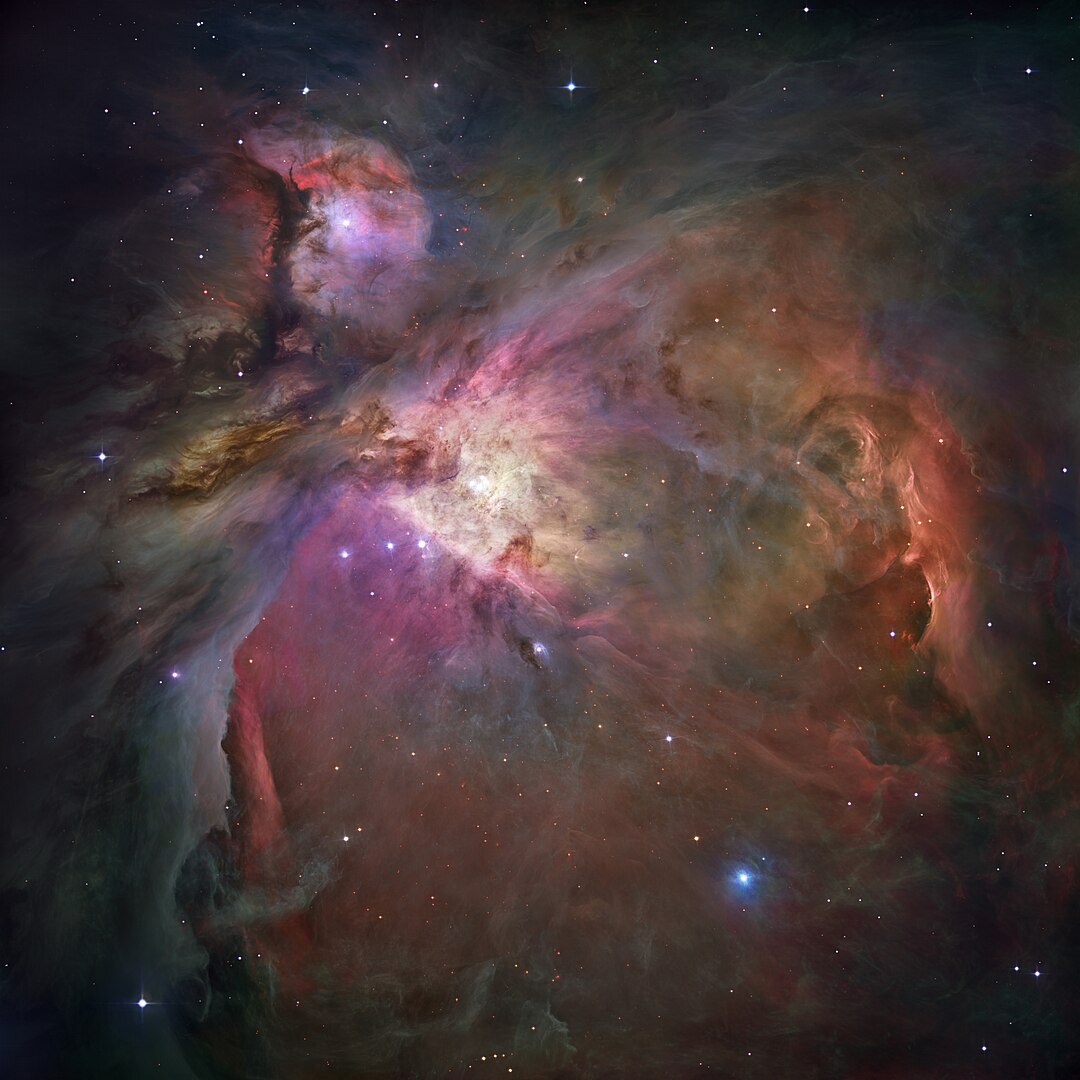
\includegraphics[width=0.85\linewidth]{Orion_Nebula_-_Hubble_2006_mosaic_1080px}
      	}
    \end{minipage}%
    \begin{minipage}{.5\linewidth}
        \centering
        \subfloat[Eagle Nebula (Messier 16) \cite{eagle_nebula_eso_2009}]{
            \label{:b}
            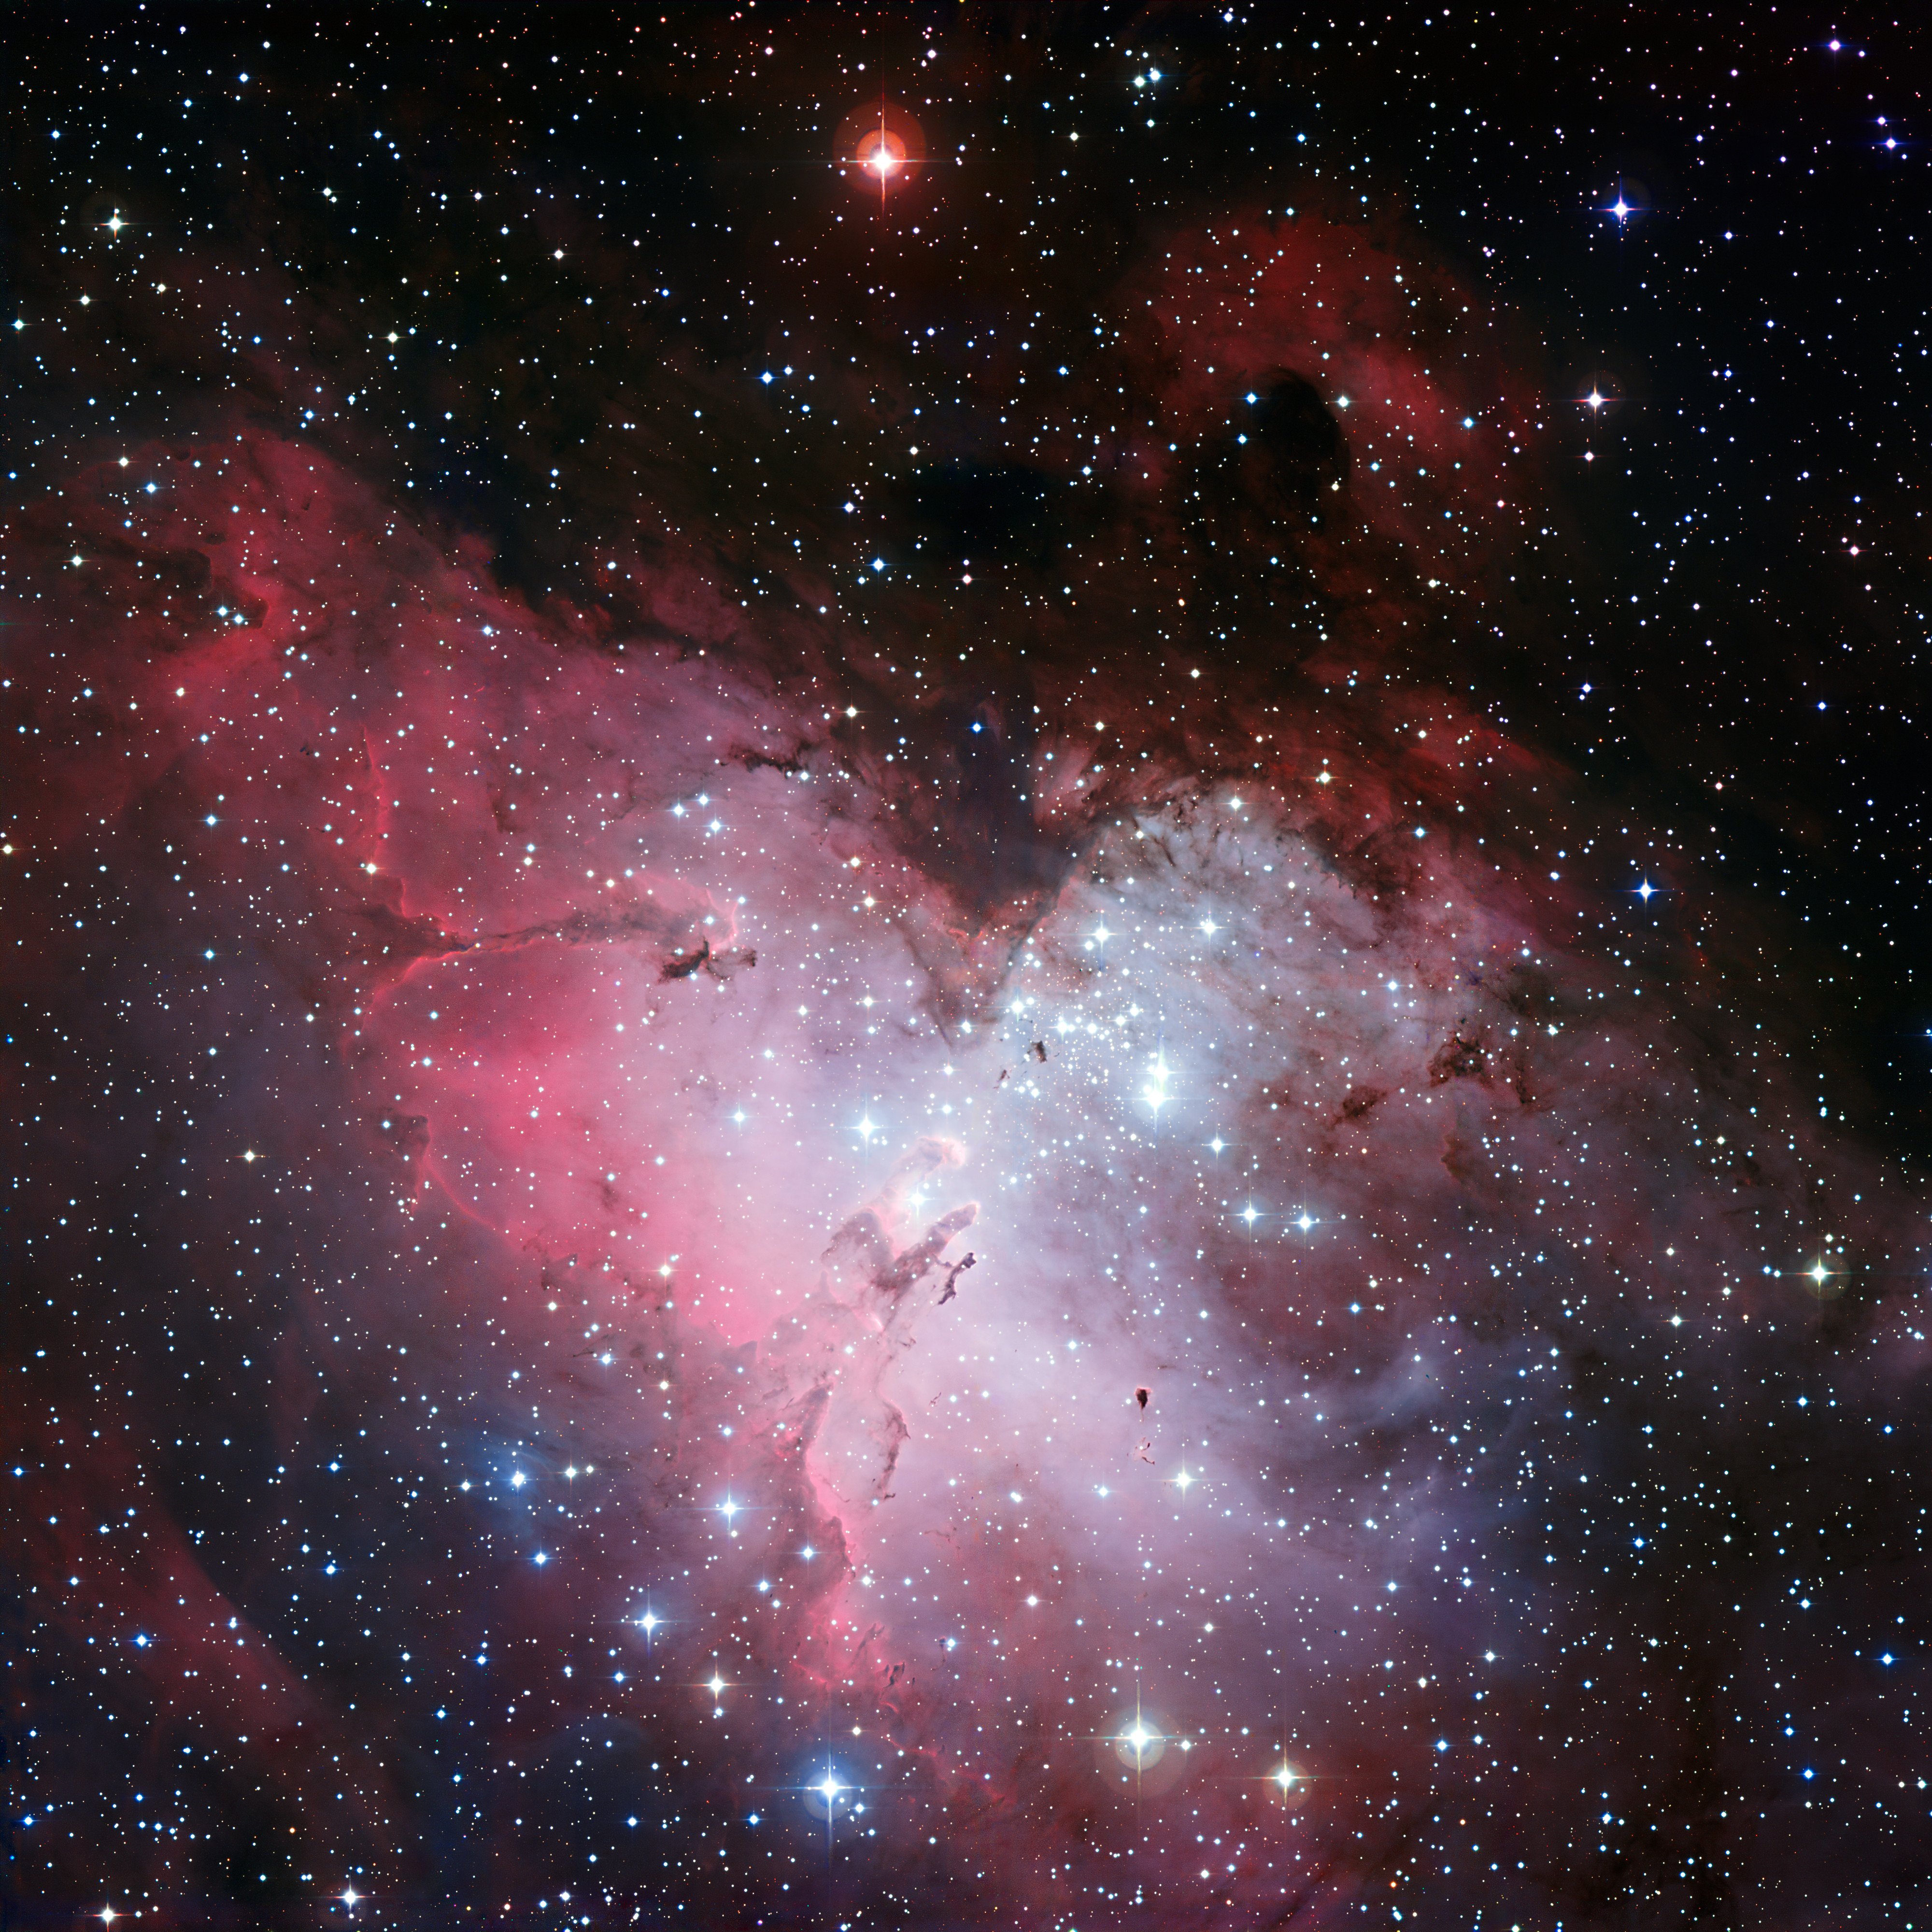
\includegraphics[width=0.85\linewidth]{eso0926a.jpg}
      	}
    \end{minipage}
    \caption{Examples of star-forming regions: (a) The Orion Nebula (b) The Eagle Nebula
        (Zoom in to see the famous \textit{Pillars of Creation} at the center of the image).
    }
    \label{fig:star_forming_regions}
\end{figure}


    % The material making up these clouds can be classified into three main categories:
    % \begin{enumerate}
    %     \item Molecular Gas: \\
    %         \todo{Mostly diatomic hydrogen $\text{H}_2$.} \\
    %         \todo{some helium, lithium, and trace amounts of heavier elements.}
    %     \item Ionized Gas: (Plasma) \\ 
    %         \todo{}
    %     \item Dust: \\
    %         \todo{Agglomerates of ...} \\
    %         \todo{held together (weakly) by ...} \\
    %         \todo{Shape: (fractal?)}
    % \end{enumerate}

    Now that we've taken a brief look at the material make-up and particle density of the ISM, 
    let us turn our attention to the question of how PPDs, stars, and planets can be formed 
    from the aforementioned clouds of gas and dust.

  % }}}
% The Nebular Hypothesis {{{ 
\clearpage\subsection{The Nebular Hypothesis}

    The \textit{nebular hypothesis} is a widely accepted model for explaining the formation and 
    evolution of not only our own Solar System, but the planetary systems around other stars as 
    well. 

    It was postulated independently by Immanuel Kant        % TODO cite
    and Pierre-Simon Laplace                                % TODO cite
    in 1755 and 1796, respectively. \\                      % TODO "independently" is that true?

    The hypothesis is built upon the idea that the formation of proto-planetary disks (and thus 
    solar systems) can be explained via the gravitational collapse of giant interstellar clouds 
    of gas and dust. (\todo: Examples for such star-forming regions, see above [cite]) \\
    \todo{(molecular clouds)}

    \todo{What is there at the beginning?}
    \begin{itemize}
        \item a giant cloud of (mostly) gas in the interstellar medium 
              (as said before: mostly di-atomic hydrogen, and mono-atomic helium)
    \end{itemize}
    \todo{How big is such a cloud?}
    \begin{itemize}
        \item ...
    \end{itemize}
    \todo{What happens?}
    \begin{itemize}
        \item The cloud collapses under its own gravity. \todo{Cause?}
        \item The cloud posseses a total angular momentum. It is most likely $\neq 0$.
        \item Therefore, the cloud does not just simply collapse into a single point. 
              (\todo{...})
        \item The cloud flattens into a disk.
        \item The majority of the mass present in the cloud gathers in the center.
        \item The rest of the mass flattens into a disk orbiting the star 
              (later: solar system).
        \item In the center/core, density and temperature increase to a point that nuclear 
              fusion becomes possible.
    \end{itemize}

    \todo{Result: PPD} \\
    \todo{Images of PPDs.}

% }}}
% The Road from Dust to Planet {{{ 
\clearpage\subsection{The Road from Dust to Planet}

    \todo{Evolution over many orders of magnitude.} \\
    \todo{Start with gas.}

    \todo{Then: dust particles}
    \begin{itemize}
        \item How do they form?
    \end{itemize}

    \todo{Then: dust agglomerates}
    \begin{itemize}
        \item They form via Coulomb and/or Van-der-Waals interactions
        \item Particles collide and, under the right circumstances, stick together.
        \item Larger and larger agglomerates form.
        \item They possess a fractal shape (dust bunnies).
    \end{itemize}
    \todo{Image of dust bunnies/fractals.}

    \todo{Then: pebbles} \\
    \todo{Then: planetesimals} \\
    \todo{Then: planetary cores (may start accreting gas)} \\
    \todo{Then: terrestrial planets} \\
    \todo{Then: gas giants (outer regions?)} \\

    \todo{Visualize particle coagulation.}

% }}}
% Preliminary Notes on Axis Discretization {{{
\clearpage\section{Preliminary Notes on Axis Discretization}
\label{sec:preliminary_notes_on_axis_discretization}

    Throughout this thesis, we will deal with several physical quantities carrying values that 
    range across many orders of magnitude. Most notably, these are time, distance, and mass. \\

    The Smoluchowski equation serves as the foundation for the coagulation model that we will 
    build. Since this integro-differential equation has analytical solutions in only a limited 
    set of cases, it will be necessary to make use of numerical integration techniques to obtain 
    an approximate solution for the evolution of the dust particle mass distribution in the 
    considered disk region. Before numerical integration, the axes for the above-mentioned 
    physical quantities will have to be discretized in an appropriate manner. \\

    As an example, we will here demonstrate how one might do this for the mass axis $m$. 
    The construction  of a discrete axis for both space (i.e. radial distance $r$ from the 
    central star) and time $t$ can then be done entirely analogously. \\

    The continuous range $m$ of particle masses present in the disk is partitioned into a set of 
    $\mathcal N_m\in\mathbb N$ intervals, which we will refer to as "bins" from this point onwards. 
    Each of these bins can be uniquely characterized by an index 
    $i\in[1,\mathcal N_m]\cap\mathbb N$, and assigned a corresponding mass value $m_i^\text{c}$, 
    which is situated at the \textit{center of the bin} (ergo the superfix "c").\\
    
    To derive an expression that can be used to calculate the mass values at these bin centers, 
    let us first define the mass values at the \textit{boundaries of the bin}. To do this,
    consider a collection of $\mathcal N_m+1$ appropriately spaced grid points $m_i^\text{b}$. 
    The first and last of these values, i.e. the lower and upper boundaries of the discrete mass 
    grid, shall be labeled $m_\text{min}$ and $m_\text{max}$, respectively. \\

    The spacing of the grid points of course depends heavily on the utilized scaling. In
    \cref{subsec:axis_discretization_with_linear_scale} and
    \cref{subsec:axis_discretization_with_logarithmic_scale}, we will go into more detail on how 
    exactly the values for $m_i^\text{b}$ and $m_i^\text{c}$ are to be defined when making use of 
    a linear and logarithmic scaling, respectively. \\
    % TODO Assure consistent usage of \text{b} and \text{c}.

    For the moment, a schematic represenation of the continuous mass axis and its discrete analogon
    can be seen visualized in \cref{fig:continuous_and_discrete_mass_axis} below.
    % TODO Display `Figure` instead of `fig`.

    \vfill

\begin{figure}[h!]
    \begin{center}
        \begin{tikzpicture}
            \def\N{5}      % This is the number of cells drawn (to the left of "..." separator).
            \def\M{6}      % This is the number of boundary arrows drawn (left of "...").
            \def\W{1.5}    % This is a cell's width.
            \def\H{\W}     % This is a cell's height.
            \def\L{\W/4}   % This is an arrow's length.
            \def\P{\W/8}   % This is the padding between arrow & cell.
            \def\R{\W/32}  % This is the padding between arrow & text.

            % Draw continuous mass axis.
            \draw [|-to](0, 2.5*\H) -- (\N*\W+4*\W, 2.5*\H);
            \draw [-](\W, 2.45*\H) -- (\W, 2.55*\H);
            \draw [-](\N*\W+3*\W, 2.45*\H) -- (\N*\W+3*\W, 2.55*\H);
            \node[] at (-2*\P, 2.5*\H) {$0$};
            \node[] at (\N*\W+4*\W+2*\P, 2.5*\H) {$m$};

            % Draw arrow from continuous to discretized mass axis.
            % \node[] at (\N*\W/2+1.5*\W, 2.25*\H) {$\Downarrow$};

            % Draw cells...
            % ...to the left of "..." separator.
            \foreach \x in {1, ..., \N} {
                \draw[draw=black] (\x*\W, 0) rectangle ++(\W, \H);
            }
            % ...to the right of "..." separator.
            \draw[draw=black] (\N*\W+2*\W, 0) rectangle ++(\W, \H);

            % Draw crosses...
            % ...to the left of "..." separator.
            \foreach \x in {1, ..., \N} {
                \draw (\x*\W+\W/2, \H/2) node {\tiny x};
            }
            % ...to the right of "..." separator.
            \draw (\N*\W+2.5*\W, \H/2) node {\tiny x};

            % Draw "..." separator.
            \node[] at (\N*\W+1.5*\W, \H/2) {...};

            % Draw arrows labeling cell boundaries.
            \foreach \x in {1, ..., \M} {
                \draw [-to](\x*\W, \H+\L+\P) -- (\x*\W, \H+\P);
                \node[] at (\x*\W, \H+\L+\P+\L+\R) {$m_\x^\text{b}$};
            }
            \draw [-to](\N*\W+2*\W, \H+\L+\P) -- (\N*\W+2*\W, \H+\P);
            \draw [-to](\N*\W+3*\W, \H+\L+\P) -- (\N*\W+3*\W, \H+\P);
            \node[] at (\N*\W+2*\W, \H+\L+\P+\L+\R) {$m_{\mathcal N_m}^\text{b}$};
            \node[] at (\N*\W+3*\W, \H+\L+\P+\L+\R) {$m_{\mathcal N_m+1}^\text{b}$};

            % Draw arrows labeling cell centers.
            \foreach \x in {1, ..., \N} {
                \draw [-to](\x*\W+\W/2, 0-\L-\P) -- (\x*\W+\W/2, 0-\P);
                \node[] at (\x*\W+\W/2, 0-\L-\P-\L-\R) {$m_\x^\text{c}$};
            }
            \draw [-to](\N*\W+2.5*\W, 0-\L-\P) -- (\N*\W+2.5*\W, 0-\P);
            \node[] at (\N*\W+2.5*\W, 0-\L-\P-\L-\R) {$m_{\mathcal N_m}^\text{c}$};

            % Draw labels for `m_min` and `m_max`.
            \node[] at (\W, \H+\L+\P+\L+3*\R+\L+\L) {$m_\text{min}$};
            \node[] at (\N*\W+3*\W, \H+\L+\P+\L+3*\R+\L+\L) {$m_\text{max}$};
            \node[] at (\W, \H+\L+\P+\L+2*\R+\L) {$=$};
            \node[] at (\N*\W+3*\W, \H+\L+\P+\L+2*\R+\L) {$=$};
        \end{tikzpicture}
    \end{center}
    \caption{Schematic illustration of the discretized mass axis. After having defined a minimum 
        value $m_\text{min}$ and a maximum value $m_\text{max}$, the interval between these two 
        values is divided evenly into $\mathcal N_m$ bins. To do this, we first define the mass
        values at the bin boundaries and, from that, the mass values at the bin centers. 
        This can be done using either a linear or a logarithmic scaling (for details, see section
        [cite linear] and [cite logarithmic], respectively). The discretization of the 
        axes for both time $t$ and distance $r$ from the star is done completely analogously.}
    \label{fig:continuous_and_discrete_mass_axis}
\end{figure}


    % Axis Discretization with Linear Scaling {{{ 
    \subsection{Axis Discretization with Linear Scaling}
    \label{subsec:axis_discretization_with_linear_scale}

        For the sake of simplicity, let us assume a linear scaling at the moment. Later on, we 
        will make use of a logarithmic scaling instead, which will help us assure a more 
        appropriate representation of all values along the wide range of dust particle masses 
        that are present in the proto-planetary disk. \\
    
        For a given bin, which can be characterized by an index $i$, the mass value corresponding 
        to this bin's lower boundary shall be labeled $m_i^\text{b}$. When using a linear scaling,
        it can be expressed as
        \begin{align}
          m_i^\text{b}=m_\text{min}+(m_\text{max}-m_\text{min})\cdot\frac{i}{\mathcal N_m}
        \end{align}

        Having derived the mass values at the boundaries of each bin, it is now quite easy to 
        calculate the corresponding values at the bin center. To do this, all we need to do is take 
        the arithmetic mean of the two boundary values:
        \begin{equation}
            m_i^\text{c}
                =\frac{m_i^\text{b}+m_{i+1}^\text{b}}{2}
        \end{equation}
        
        Thus, after having defined only the three numbers $\mathcal N_m$, $m_\text{min}$, and 
        $m_\text{max}$, it is possible to interpolate the values of all mass grid points positioned 
        on both the boundaries as well as the  centers of the bins. \\
        
        The inverse transformation from mass to index can be derived easily by rearranging the 
        above relation, which leads to the following expression:
        \begin{equation}
            i(m)
                =\mathcal N_m\cdot\frac{m-m_\text{min}}{m_\text{max}-m_\text{min}}
        \end{equation}
        
        % Sidenote: In the linearily scaled mass grid, the bin "width" is constant, and independent of the 
        % bin index. This will change once the switch to a logarithmic grid is made! For now though, it is 
        % given by
        % \begin{align}
        %   \Delta m
        %   &=m_{i+1}^\text{b}-m_i^\text{b}\\
        %   &=\frac{m_\text{max}-m_\text{min}}{\mathcal N_m}
        % \end{align}
 
    % }}}
    % Axis Discretization with Logarithmic Scaling {{{ 
    \subsection{Axis Discretization with Logarithmic Scaling}
    \label{subsec:axis_discretization_with_logarithmic_scale}

        The procedure for constructing the discretized axis using a logarithmic scaling works quite
        analogously to what we just saw in the linear case. (The main difference is that we switch
        out addition/subtraction by multiplication/division, and multiplication/division by
        exponentiation.)
        \\

        As before, let $\mathcal N_m$ label the total number of bins, each of which can be uniquely 
        identified by an index $i\in\mathcal[1,\mathcal N_m+1]$. Once again, we will first define 
        an expression for the grid points sitting directly on the lower boundary of each bin. When
        making use of a logarithmic scaling, these values are given by
        \begin{equation}
            m_i^\text{b}
                =m_\text{min}\cdot\left(\frac{m_\text{max}}{m_\text{min}}\right)^{i/\mathcal N_m}
        \end{equation}
        To arrive at the mass values at the bin centers, we again take the mean. Contrary to the 
        linear case, here we are not using the arithmetic mean though, but the geometric mean
        instead:
        \begin{align}
            m_i^\text{c}
                =\sqrt{m_i\cdot m_{i+1}}
        \end{align}
    
        As in the linear case, the inverse transformation can easily be arrived at by rearranging
        for the index $i$, which leads to the following expression:
        \begin{align}
            i(m) = \mathcal N_m\cdot \frac{
                \log(m)-\log(m_\text{min})
            }{
                \log(m_\text{max})-\log(m_\text{min})
            }
        \end{align}
        
        In contrast to the linear grid, where the "bin width", i.e. the additive offset between bins
        \begin{equation}
            \Delta m := m_{i+1} - m_i
        \end{equation}
        is the same for all bins, in the logarithmic grid this is not the case. Instead, what stays
        constant here is the \textit{relative} mass increase from one bin to the next:\footnote{This
        is true only up to the machine precision of the utilized computer setup.}
        \begin{equation}
            \frac{m_i^\text{c}}{m_i^\text{c}}
                =\frac{m_i^\text{b}}{m_i^\text{b}}
                =\text{const.}\ \forall i\in[1,\mathcal N_m]
        \end{equation}

    % }}}

% }}}
% Preliminary Notes on the Dust Model {{{ 
\clearpage\section{Preliminary Notes on the Dust Model}
\label{sec:preliminary_notes_on_the_dust_model}

% A Single Dust Particle {{{ 

    Let us now turn our attention to individual dust particles: \\

    % \assume{
    In the context of this thesis, we will model the individual dust particles as perfectly 
    spherical bodies of a shared solid density $\rho_s$. This allows us to group the particles 
    into different classes, each uniquely identified by the particles' mass value $m$.
    Also, this shape allows us state the following relationship between particle mass and 
    particle radius $a$:
    % }
    \begin{align}
        m
            =\rho_s \cdot \frac{4\pi}{3}a^3
        \ \ \ \ \ \text{and}\ \ \ \ \
        a
            =\bigg(\frac{3}{4\pi} \cdot \frac{m}{\rho_s}\bigg)^{1/3}
    \end{align}

    Building upon prior work done by Birnstiel, Dullemond, \& Brauer % TODO Use Oxford comma?
    \cite{birnstiel_dullemond_brauer_2010}, we will assume that the volume density of the dust 
    particles carries a value of
    $$\rho_s=\SI{1600}{\kilogram\ \meter^{-3}}$$
    % TODO Increase spacing in `\SI` renders, here & elsewhere.

    \begin{figure}[h!]
        \centering
        \begin{minipage}{.5\linewidth}
            \centering
          	\subfloat[Compact]{
                \label{:a}
                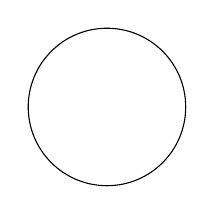
\begin{tikzpicture}
                    \def\R{1}
                    \draw[fill={black!0!white}] (0, 0) circle (\R);
                \end{tikzpicture}
          	}
        \end{minipage}%
        \begin{minipage}{.5\linewidth}
            \centering
          	\subfloat[Porous (BPCA)]{
                \label{:b}
                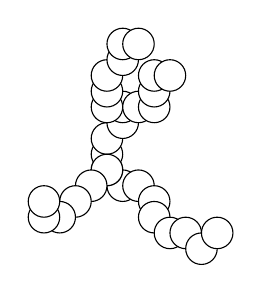
\begin{tikzpicture}
                    \def\R{0.2}
                    \draw[fill={black!0!white}] ( 1*\R, -1*\R) circle (\R);
                    \draw[fill={black!0!white}] ( 2*\R, -1*\R) circle (\R);
                    \draw[fill={black!0!white}] ( 3*\R, -2*\R) circle (\R);
                    \draw[fill={black!0!white}] ( 3*\R, -3*\R) circle (\R);
                    \draw[fill={black!0!white}] ( 4*\R, -4*\R) circle (\R);
                    \draw[fill={black!0!white}] ( 5*\R, -4*\R) circle (\R);
                    \draw[fill={black!0!white}] ( 6*\R, -5*\R) circle (\R);
                    \draw[fill={black!0!white}] ( 7*\R, -4*\R) circle (\R);

                    \draw[fill={black!0!white}] ( 0*\R,  0*\R) circle (\R);
                    \draw[fill={black!0!white}] ( 0*\R,  1*\R) circle (\R);
                    \draw[fill={black!0!white}] ( 0*\R,  2*\R) circle (\R);
                    \draw[fill={black!0!white}] ( 1*\R,  3*\R) circle (\R);
                    \draw[fill={black!0!white}] ( 1*\R,  4*\R) circle (\R);

                    \draw[fill={black!0!white}] ( 0*\R,  4*\R) circle (\R);
                    \draw[fill={black!0!white}] ( 0*\R,  5*\R) circle (\R);
                    \draw[fill={black!0!white}] ( 0*\R,  6*\R) circle (\R);
                    \draw[fill={black!0!white}] ( 1*\R,  7*\R) circle (\R);
                    \draw[fill={black!0!white}] ( 1*\R,  8*\R) circle (\R);
                    \draw[fill={black!0!white}] ( 2*\R,  8*\R) circle (\R);

                    \draw[fill={black!0!white}] ( 2*\R,  4*\R) circle (\R);
                    \draw[fill={black!0!white}] ( 3*\R,  4*\R) circle (\R);
                    \draw[fill={black!0!white}] ( 3*\R,  5*\R) circle (\R);
                    \draw[fill={black!0!white}] ( 3*\R,  6*\R) circle (\R);
                    \draw[fill={black!0!white}] ( 4*\R,  6*\R) circle (\R);

                    \draw[fill={black!0!white}] ( 0*\R,  0*\R) circle (\R);
                    \draw[fill={black!0!white}] (-1*\R, -1*\R) circle (\R);
                    \draw[fill={black!0!white}] (-2*\R, -2*\R) circle (\R);
                    \draw[fill={black!0!white}] (-3*\R, -3*\R) circle (\R);
                    \draw[fill={black!0!white}] (-4*\R, -3*\R) circle (\R);
                    \draw[fill={black!0!white}] (-4*\R, -2*\R) circle (\R);
                \end{tikzpicture}
          	}
        \end{minipage}
        \begin{minipage}{.5\linewidth}
            \centering
          	\subfloat[Fractal (BCCA)]{
                \label{:a}
                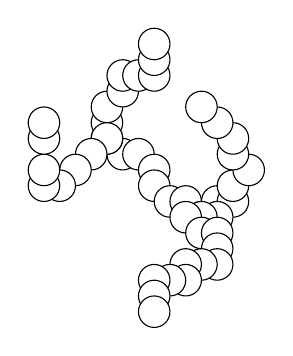
\begin{tikzpicture}
                    \def\R{0.2}
                    \draw[fill={black!0!white}] ( 1*\R, -1*\R) circle (\R);
                    \draw[fill={black!0!white}] ( 2*\R, -1*\R) circle (\R);
                    \draw[fill={black!0!white}] ( 3*\R, -2*\R) circle (\R);
                    \draw[fill={black!0!white}] ( 3*\R, -3*\R) circle (\R);
                    \draw[fill={black!0!white}] ( 4*\R, -4*\R) circle (\R);
                    \draw[fill={black!0!white}] ( 5*\R, -4*\R) circle (\R);
                    \draw[fill={black!0!white}] ( 6*\R, -5*\R) circle (\R);
                    \draw[fill={black!0!white}] ( 7*\R, -4*\R) circle (\R);
                    \draw[fill={black!0!white}] ( 8*\R, -4*\R) circle (\R);
                    \draw[fill={black!0!white}] ( 8*\R, -3*\R) circle (\R);
                    \draw[fill={black!0!white}] ( 9*\R, -2*\R) circle (\R);
                    \draw[fill={black!0!white}] ( 8*\R, -1*\R) circle (\R);
                    \draw[fill={black!0!white}] ( 8*\R,  0*\R) circle (\R);
                    \draw[fill={black!0!white}] ( 7*\R,  1*\R) circle (\R);
                    \draw[fill={black!0!white}] ( 6*\R,  2*\R) circle (\R);
                    \draw[fill={black!0!white}] ( 7*\R, -5*\R) circle (\R);
                    \draw[fill={black!0!white}] ( 6*\R, -5*\R) circle (\R);
                    \draw[fill={black!0!white}] ( 5*\R, -5*\R) circle (\R);
                    \draw[fill={black!0!white}] ( 6*\R, -6*\R) circle (\R);
                    \draw[fill={black!0!white}] ( 7*\R, -6*\R) circle (\R);
                    \draw[fill={black!0!white}] ( 7*\R, -7*\R) circle (\R);
                    \draw[fill={black!0!white}] ( 7*\R, -8*\R) circle (\R);

                    \draw[fill={black!0!white}] ( 6*\R, -8*\R) circle (\R);
                    \draw[fill={black!0!white}] ( 5*\R, -8*\R) circle (\R);
                    \draw[fill={black!0!white}] ( 5*\R, -9*\R) circle (\R);
                    \draw[fill={black!0!white}] ( 4*\R, -9*\R) circle (\R);
                    \draw[fill={black!0!white}] ( 3*\R, -9*\R) circle (\R);
                    \draw[fill={black!0!white}] ( 3*\R, -10*\R) circle (\R);
                    \draw[fill={black!0!white}] ( 3*\R, -11*\R) circle (\R);

                    \draw[fill={black!0!white}] ( 0*\R,  0*\R) circle (\R);
                    \draw[fill={black!0!white}] ( 0*\R,  1*\R) circle (\R);
                    \draw[fill={black!0!white}] ( 0*\R,  2*\R) circle (\R);
                    \draw[fill={black!0!white}] ( 1*\R,  3*\R) circle (\R);
                    \draw[fill={black!0!white}] ( 1*\R,  4*\R) circle (\R);
                    \draw[fill={black!0!white}] ( 2*\R,  4*\R) circle (\R);
                    \draw[fill={black!0!white}] ( 3*\R,  4*\R) circle (\R);
                    \draw[fill={black!0!white}] ( 3*\R,  5*\R) circle (\R);
                    \draw[fill={black!0!white}] ( 3*\R,  6*\R) circle (\R);

                    \draw[fill={black!0!white}] ( 0*\R,  0*\R) circle (\R);
                    \draw[fill={black!0!white}] (-1*\R, -1*\R) circle (\R);
                    \draw[fill={black!0!white}] (-2*\R, -2*\R) circle (\R);
                    \draw[fill={black!0!white}] (-3*\R, -3*\R) circle (\R);
                    \draw[fill={black!0!white}] (-4*\R, -3*\R) circle (\R);
                    \draw[fill={black!0!white}] (-4*\R, -2*\R) circle (\R);
                    \draw[fill={black!0!white}] (-4*\R,  0*\R) circle (\R);
                    \draw[fill={black!0!white}] (-4*\R,  1*\R) circle (\R);
                \end{tikzpicture}
          	}
        \end{minipage}%
        \begin{minipage}{.5\linewidth}
            \centering
          	\subfloat[Linear]{
                \label{:b}
                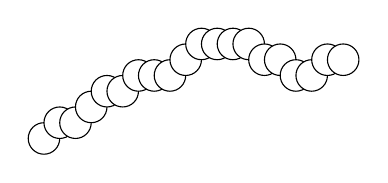
\begin{tikzpicture}
                    \def\R{0.2}
                    \draw[fill={black!0!white}] ( 0*\R,  0*\R) circle (\R);
                    \draw[fill={black!0!white}] ( 1*\R,  1*\R) circle (\R);
                    \draw[fill={black!0!white}] ( 2*\R,  1*\R) circle (\R);
                    \draw[fill={black!0!white}] ( 3*\R,  2*\R) circle (\R);
                    \draw[fill={black!0!white}] ( 4*\R,  3*\R) circle (\R);
                    \draw[fill={black!0!white}] ( 5*\R,  3*\R) circle (\R);
                    \draw[fill={black!0!white}] ( 6*\R,  4*\R) circle (\R);
                    \draw[fill={black!0!white}] ( 7*\R,  4*\R) circle (\R);
                    \draw[fill={black!0!white}] ( 8*\R,  4*\R) circle (\R);
                    \draw[fill={black!0!white}] ( 9*\R,  5*\R) circle (\R);
                    \draw[fill={black!0!white}] (10*\R,  6*\R) circle (\R);
                    \draw[fill={black!0!white}] (11*\R,  6*\R) circle (\R);
                    \draw[fill={black!0!white}] (12*\R,  6*\R) circle (\R);
                    \draw[fill={black!0!white}] (13*\R,  6*\R) circle (\R);
                    \draw[fill={black!0!white}] (14*\R,  5*\R) circle (\R);
                    \draw[fill={black!0!white}] (15*\R,  5*\R) circle (\R);
                    \draw[fill={black!0!white}] (16*\R,  4*\R) circle (\R);
                    \draw[fill={black!0!white}] (17*\R,  4*\R) circle (\R);
                    \draw[fill={black!0!white}] (18*\R,  5*\R) circle (\R);
                    \draw[fill={black!0!white}] (19*\R,  5*\R) circle (\R);
                \end{tikzpicture}
          	}
        \end{minipage}
        \caption{
            \todo{in reality, fractals [image!]} \\ 
            \todo{in our case, spheres}
        }
        \label{}
    \end{figure}


% }}}
% Continuous Formulation {{{ 
\clearpage\subsection{The Dust Particle Mass Distribution Function}
\label{sec:dust_particle_mass_distribution}

    The concept of the \textit{dust particle mass distribution function} $n(m, \vec r, t)$ 
    lies at the heart of the dust coagulation model that was built for this thesis. 
    This function is defined in such a way that, at a given time $t$ and position $\vec r$ 
    in the disk, the expression
    \begin{equation}
        N(\vec r, t) =\int\limits_0^\infty n(m,\vec r, t)\ \dd m
    \end{equation}
    denotes the total number of dust particles $N$ per unit volume, i.e. the dust particle
    number density, at the considered region in the proto-planetary disk. 
    Its relationship to the dust mass volume density $\rho_d$ at a given position $\vec r$ 
    in the disk is given by
    \begin{equation}
        \label{eq:relationship_between_dust_particle_mass_distribution_and_mass_volume_density}
        % \rho_\text{dust} = 
        \rho_d(\vec r) =\int\limits_0^\infty n(m,\vec r, t)\cdot m\ \dd m
    \end{equation}

    % The temporal evolution of the functions $n$, $N$, and $\rho_g$ will be of great interest 
    % throughout this thesis.

% }}}
% Discretized Formulation {{{ 
% \subsection{Discretized Formulation}

    Before we can use numerical integration techniques to calculate an approximate solution to 
    the Smoluchowski coagulation equation, it will be necessary to define an analogous, 
    but discretized formulation of the expressions we defined above. \\

    Let $m_i$ label the discretized mass axis we already defined in
    \cref{sec:preliminary_notes_on_axis_discretization}
    (\todo{specifically $m_i^c$}).
    As before, the mass grid consists of $\mathcal N_m$ bins, with an lower and upper axis 
    boundary $m_\text{min}$ and $m_\text{max}$, respectively. The mass "width" of a given bin 
    at a position $i$ in the grid is labeled $\Delta m_i$. \\

    We will begin with the discretized particle mass distribution functions.
    For this, let us introduce the notation
    \begin{equation}
        \label{eq:discrete_formulation_of_particle_mass_distribution}
        n_i := n(m_i)
    \end{equation}

    The total number of dust particles per unit unit volume belonging to a given bin $i$ is 
    then calculated by integrating the particle mass distribution function from the lower to 
    the upper bin boundary:
    \begin{align}
        \label{eq:relationship_between_dust_particle_mass_distribution_and_particle_number_density}
        N_i 
        &= \int_{m_{i-1/2}}^{m_{1+1/2}}n(m)\ \dd m \\
        &\approx n_i \cdot \Delta m_i 
        % \ \ \ \textcolor{red}{??}
    \end{align}
    
    The mass density $\rho_i$ in the bin $i$ is given by
    \begin{align}
        \label{eq:relationship_between_discretized_dust_particle_mass_distribution_and_mass_volume_density}
        \rho_i 
        &= \int_{m_{i-1/2}}^{m_{1+1/2}} m \cdot n(m)\ \dd m \\
        &\approx n_i \cdot m_i \cdot \Delta m_i 
    \end{align}
    
    Each bin in the mass grid contains a certain fraction of the total dust mass density
    $\rho_d(\vec r)$ at a given point $\vec r$ in space. 
    Therefore, to arrive at the total mass density independent of particle mass, 
    one has to sum over all bins:
    \begin{align}
      \rho=\sum_{i=1}^{\mathcal N_m} \rho_i
    \end{align}
    % TODO Make approximation here? Need to switch from integral to sum at some point.

    In the context of this thesis, we will study the temporal evolution of 
    \todo{but $\rho_d$ is constant. (mass conservation)}

% }}}
% Initialization of the Dust Mass Distribution {{{ 
\clearpage\subsection{Initialization of the Dust Mass Distribution}

    Let us label the initial state of the dust particle mass distribution function and particle
    number density
    \begin{align}
        n_0 &:= n(m=m_0, t=0) 
        \ \ \ \ \text{and}\ \ \ \
        \\
        N_0 &:= N(m=m_0, t=0)
    \end{align}
    respectively. \\

    At the beginning of a given simulation, we will assume all dust particles to share the same 
    mass $m_0$ and the same corresponding radius.
    The appropriate particle mass distribution function for the this scenario is a 
    Dirac $\delta$-distribution:
    \begin{equation}
        \label{eq:dirac_delta_identity}
        n(m, \vec r, t=0) = \delta_D(m-m_0) \cdot n_0  
    \end{equation}
    % Here, the normalization constant $n_0$ is the initial number of particles 
    % with mass $m_0$ per unit volume. NO!
    % TODO assume large scale dust density does stay constant

    Plugging the above definition back into
    \cref{eq:relationship_between_dust_particle_mass_distribution_and_mass_volume_density}
    leads to
    \begin{align}
        \rho_d(\vec r) 
            &= \int\limits_{-\infty}^\infty n(m, \vec r, t) \cdot m\ \text dm \\
            &= \int\limits_{-\infty}^\infty \delta_D(m-m_0) \cdot n_0 \cdot m\ \text dm \\
            &= N_0 \cdot m_0
    \end{align}
    This reflects the fact that we initially want to have $N_0$ particles per unit volume, each 
    carrying a mass of value $m_0$. \\

    Implementing this numerically means defining a vector of length $\mathcal N_m$, consisting of 
    $\mathcal N_m-1$ zeros and a single non-zero entry.
    We have to define a discretized analogon of the above.
    \begin{equation}
        n_i(t=0) = \delta_{ij} \cdot n_0
    \end{equation}
    Plugging this back into 
    \cref{eq:relationship_between_discretized_dust_particle_mass_distribution_and_mass_volume_density}
    yields
    \begin{align}
        \rho_d 
            &= \sum_{i=1}^{\mathcal N_m} n_i \cdot m_i \cdot \Delta m_i \\
            &= \sum_{i=1}^{\mathcal N_m} \delta_{ij} \cdot n_0 \cdot m_i \cdot \Delta m_i \\
            &= \cdot n_0 \cdot m_j \cdot \Delta m_j
    \end{align}

    % \begin{equation}
    %     n_i \cdot m_i \cdot \Delta m_i = \rho_d
    % \end{equation}

    If not specified otherwise, the initial particle mass will be set to $m_0 = m_c^1$ for the
    remainder of this thesis. This is the mass value at the center of the first ("smallest") bin 
    in the discrete mass grid.

    % that no coagulation or fragmentation 
    % has taken place so far

    % \todo{At the beginning, assume no coagulation has taken place (at all?).} \\
    % \todo{Write about formation of smallest dust grains: From ISM? Formed from gas in disk?} \\

    % \todo{All particles have lowest possible mass.} \\
    % \todo{Mass distribution function is initialized as Dirac delta distribution centerd on 
    % "lowest bin".} \\

    % \todo{Add plot.}

% }}}

% }}}





































    % \item Dust plays an important role in the process of planet formation.

% Immediately after the Big Bang, 
% In this work, we will examine the feasibility of using Monte Carlo kernel sampling 
% to lower the computational cost of integrating the Smoluchowski coagulation equation.
% The disk model is defined in \cref{ch:disk}.
% The coagulation model is defined in \cref{ch:smoluchoswki}.
% In \cref{ch:sampling}, we implement stochastic sampling of collision pairs,
% to lower the number of kernel matrix terms that one has to sum over in 
% each time step.
% Before we will start with the definition of the disk, the following attempts to provide 
% a brief overview over ...
% The thesis will be structured in the following way:
% We will start with the definition of a simple disk model, 
% which includes some of the most relevant properties of 
% both the disk, as well as its gas and dust contents.
% From that we will derive expressions for the 
% collisions

% Then, we sample

% In this work, we deal a lot with dust

% Question: Where did everything come from?

% \section{Brief Overview}

% Directly after the Big Bang, the conditions were not given for large-scale structure formation.

% The universe was too hot for large structure formation in the times immediately 
% following the Big Bang. 
% As the quark-gluon plasma cooled down with the expansion of the universe, 

% the formation of first hadrons (proton, neutron) from their quark "components/consituents",
% then 
 
% Immediately after the Big Bang
% After the Big Bang, the universe was filled with a hot quark-gluon plasma [cite].

% For the first [\todo{?}] after the Big Ban

% \section{todos}

% In this work, we will examine the feasibility of using Monte Carlo kernel sampling 
% to lower the computational cost of integrating the Smoluchowski coagulation equation.

% Before we can to that, we have to "introduce a number of concepts".
% The following provides a brief overview over the way this thesis is structured.

% Since we are trying to model the temporal evolution of the mass distribution of 
% dust particles in a proto-planetary disk, it will be necessary to define a disk model,
% including the "most relevant" properties of the disk itself as well as its gas and dust contents.
% \cref{ch:disk}

% - the Smoluchowski coagulation equation
% - Monte Carlo sampling of the kernel matrix

% Also
% - define a disk model
% - with gas and dust contents
% - dust kinematics and collisions

% % \section{intro}
% % \section{abstract}

% The coagulation of dust particles 

% % \section{00}

% The interaction of dust particles in proto-planetary disk via a combination of 
% Van der Waals and electrostatic forces is believed to play an important role 
% in the early stages of planetesimal formation inside proto-planetary disks. [cite]

% Once large enough, the gravitational influence of these bodies can 
% become strong enough to enable accretion of the surrounding gas (?), 
% and thus, planetary core formation. (?) \\


% why is dust coagulation relevant? \\
% what is the Smoluchowski equation/formalism? \\
% why kernel sampling? \\
% what is needed: disk model, collision rates, kernel definition for coagulation and fragmentation \\

% thesis structure

% model disk properties along radial axis \\
% model gas distribution along radial axis \\
% from that, dust distribution \\
% model dust particle kinematics \\
% from rel. vel. derive dust particle collision rate \\
% construct kernel for both "coagulation and fragmentation" processes \\
% examine stability properties \\
% use monte carlo sampling of relevant collisions to reduce computational complexity of integration \\

% % \section{01}
% 2
% \begin{itemize}
%     \item focus on formation of larger dust particles
%     \item particle collisions, coagulation and fragmentation
%     \item distribution of particles sizes (radii and masses)
%     \item temporal evolution of distribution modeled using framework given by the 
%           Smoluchowski coagulation equation
%     \item involves construction of kernel matrix
%     \item integration requires evaluation of multi-dimensional sum
%     \item Let $m$ be the mass of a group of particles. How does the number of particles with 
%           mass $m$ change under the influence of collisions between two particles carrying 
%           mass $m'$ and $m''$?
%     \item this information is encoded into the kernel $K(m,m',m'')$
%     \item 
% \end{itemize}

% \section{000}

% Immediately after the Big Bang the early universe was much too hot 
% to allow the formation of particles as large as what one might find 
% on Earth today.

% But with the expansion of the universe 
% the universe cooled up enough to ...

% From the "quark-gluon" plasma formed

% After the Big Bang, ...
% It took the universe ... to cool down sufficiently to allow the formation of 

% When the universe had cooled down sufficiently to allow the formation of atoms
% After the Big Bang, the universe hot 

% % \section{000}
% \begin{itemize}
%     \item Big Bang, hot universe, "quark-plasma"
%     \item universe cools down
%     \item sufficiently to allow the condensation of matter into larger structures
%     \item atoms (hydrogen), molecules (H$_2$)
%     \item star formation, fusion into heavier elements
%     \item matter "emitted" into "surrounding regions \& ISM"
%     \item dust particles form
%     \item not the kind of dust that accumulates at home
%     \item instead: \todo{carbon, oxygen, silicon, ?}
% \end{itemize}

% The goal of this thesis:
% \begin{itemize}
%     \item Build a disk model.
%     \item Use that disk model to define particle collision rates.
%     \item Define kernel matrices for coagulation and fragmentation, with collision rate.
%     \item Use Smoluchowski equation to model temporal evolution of dust particle mass distribution.
%     \item Integrate Smoluchowski equation.
%     \item Sample collision.
% \end{itemize}

% \section{Historical Context}

%     % TODO For inspiration, see
%     % - "Theoretical Models of the Structure of Protoplanetary Disks Les Houches 2013" by Kees
%     % - Introduction of "PhD thesis" by Til Birnstiel
    
%     \todo{Question "How was Earth created" (probably) almost as old humanity itself} \\
%     \todo{"Problem/Puzzle" still not solved, lots of open questions} \\
%     \todo{We now know: Planets are "byproducts of star formation"} \\

%     \todo{Ever since the time of the earliest human civilizations, ...} \\
%     \todo{Humans have been intrigued by the ... night sky.} \\
%     \todo{Even before the invention of telescopes, with the naked eye alone...} \\
%     \todo{Several bright objects could be distinguished from the rest of the night sky} \\
%     \todo{Distinguish planets from stars, they exhibit relative motion ("planetes").} \\
%     \todo{Ptolemai: Earth as center of the universe.} \\
%     \todo{Copernicus: Sun as center of the Solar System.} \\
%     \todo{Kepler: Kepler's laws, ellipsoid trajectories.} \\
%     \todo{Newton: law of gravitation.} \\
%     \todo{Discovery of planets in our solar system.} \\
%     \todo{Discovery of exo-planets} \\
%     \todo{Question: How do planets form?}
        
% \section{Planet Formation}


% \section{Motivation for this Thesis}

%     \todo{Why is planet formation relevant to us at all?} \\
%     \todo{Why is dust coagulation relevant to planet formation?} \\
%     \todo{How can one model dust coagulation?} \\
%     \todo{What are the challenges involved in that model? (int. of Smol. eq.)} \\
%     \todo{How does this thesis help with that?} 
